\documentclass{article}
\usepackage{amsmath, sfmath, multicol, tkz-euclide, array, enumerate, tcolorbox, tabularray}
\renewcommand{\familydefault}{\sfdefault}
\setlength{\parindent}{0cm}
\pagestyle{empty}
\usepackage[left=1in, top=0.5in, right=1in, bottom=0.5in]{geometry}
\tikzset{>=stealth, label style/.append style={font=\footnotesize}}
\tcbset{colback=white}

\newcounter{example}[section]
\newenvironment{example}[1][]{\refstepcounter{example}\par\medskip
   {\color{red}\textbf{Example~\theexample. #1}}}{\medskip}

\begin{document}

\section*{Pythagorean Theorem and Its Converse}

\begin{tcolorbox}[colframe=orange!70!white, coltitle=black, title=\textbf{Today I Can}]
\begin{enumerate}
    \item Apply the Pythagorean Theorem and its converse.
\end{enumerate}
\end{tcolorbox}
\smallskip 

\begin{tcolorbox}[colframe=black!20!white, opacitybacktitle=0.1, coltitle=black, title=\textbf{Pythagorean Theorem}]

\begin{minipage}{0.5\textwidth}
\begin{itemize}
    \item If $\triangle ABC$ is a right triangle with hypotenuse $c$ and legs $a$ and $b$, then $a^2+b^2=c^2$.
\end{itemize}
\end{minipage}
\hspace{0.5in}
\begin{minipage}{0.4\textwidth}
    \begin{tikzpicture}[scale=0.6]
    \tkzDefPoints{0/0/A, 2/0/C, 2/2.1/B}
    \tkzDrawPolygon(A,B,C)
    \tkzLabelSegment[below](A,C){$b$}
    \tkzMarkRightAngle(B,C,A)
    \tkzLabelSegment[right](B,C){$a$}
    \tkzLabelSegment[above left](A,B){$c$}
    \node at (5.5,1) {$a^2 + b^2 = c^2$};
\end{tikzpicture}
\end{minipage}
\end{tcolorbox}
\smallskip 

\begin{tcolorbox}[colframe=black!20!white, opacitybacktitle=0.1, coltitle=black, title=\textbf{Pythagorean Triple}]
A set of nonzero whole numbers, $a$, $b$, and $c$ that satisfy the equation $a^2+b^2=c^2$.
\end{tcolorbox}
\smallskip 

Some common Pythagorean triples are \{3, 4, 5\}, \{5, 12, 13\}, \{8, 15, 17\}, and \{7, 24, 25\}. \newline 

\begin{example}
\begin{enumerate}[(a)]
    \item What is the length of the hypotenuse of $\triangle ABC$? Do the side lengths form a Pythagorean triple?   \newline

    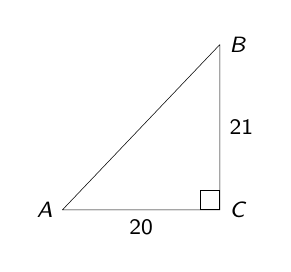
\begin{tikzpicture}
    \tkzDefPoints{0/0/A, 2/0/C, 2/2.1/B}
    \tkzDrawPolygon(A,B,C)
    \tkzLabelPoints[left](A)
    \tkzLabelPoints[right](B,C)
    \tkzLabelSegment[below](A,C){20}
    \tkzMarkRightAngle(B,C,A)
    \tkzLabelSegment[right](B,C){21}
    \end{tikzpicture}

    \item The legs of a right triangle have lengths 10 and 24. What is the length of the hypotenuse?
\end{enumerate}
\end{example}

\vspace{0.75in}

\begin{example}
Find the value of $x$ in each. Express your answer in simplest radical form (exact answer).
\begin{multicols}{2}
\begin{enumerate}[(a)]
    \item \mbox{} \newline 
    \item \mbox{} \newline 
\end{enumerate}
\end{multicols}
\begin{minipage}{0.5\textwidth}
    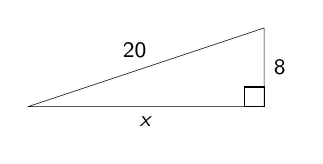
\begin{tikzpicture}
    \tkzDefPoints{0/0/A, 3/0/B, 3/1/C}
    \tkzDrawPolygon(A,B,C)
    \tkzMarkRightAngle(C,B,A)
    \tkzLabelSegment[below](A,B){$x$}
    \tkzLabelSegment[right](B,C){8}
    \tkzLabelSegment[above left,xshift=0.05in](A,C){20}
    \end{tikzpicture}
\end{minipage}
\begin{minipage}{0.4\textwidth}
    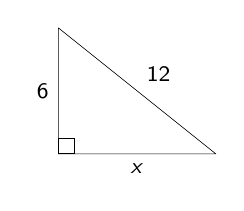
\begin{tikzpicture}[scale=0.8]
    \tkzDefPoints{0/0/C, 2.5/0/A, 0/2/B}
    \tkzDrawPolygon(A,B,C)
    \tkzMarkRightAngle(B,C,A)
    \tkzLabelSegment[below](C,A){$x$}
    \tkzLabelSegment[left](C,B){6}
    \tkzLabelSegment[above right](A,B){12}
    \end{tikzpicture}
\end{minipage}
\end{example}

\newpage 

\begin{tcolorbox}[colframe=black!20!white, opacitybacktitle=0.1, coltitle=black, title=\textbf{Converse of the Pythagorean Theorem}]
If $a^2+b^2=c^2$ then $\triangle ABC$ is a right triangle.
\end{tcolorbox}
\smallskip 

\begin{example}
\begin{enumerate}[(a)]
    \item A triangle has side lengths 13, 84, and 85. Is the triangle a right triangle? Explain.    \\[1in]
    \item A triangle has side lengths 50, 48, and 16. Is the triangle a right triangle? Explain.    \\[1.5in]
\end{enumerate}
\end{example}

\setlength{\extrarowheight}{3pt}
\begin{tabular}{c|c}
    \textbf{Obtuse Triangle} & \textbf{Acute Triangle} \\ \hline 
    longest side $^2$ $>$ smaller side $^2$ + smaller side $^2$ &
    longest side $^2$ $<$ smaller side $^2$ + smaller side $^2$ \\[3pt] \hline
    $c^2 > a^2+b^2$ &  
    $c^2 < a^2+b^2$
      
\end{tabular}

% If $c^2 > a^2+b^2$ then $\triangle ABC$ is obtuse.  \qquad
% If $c^2 < a^2+b^2$ then $\triangle ABC$ is acute.
\vspace{0.5in}

\begin{example}
Classify each of the following by its angles.
\begin{enumerate}[(a)]
    \item A triangle with side lengths 14, 11, and 6    \\[1in]
    \item A triangle with side lengths 7, 8, and 9
\end{enumerate}
\end{example}

\end{document}
